


\tikzset{every picture/.style={line width=0.75pt}} %set default line width to 0.75pt        

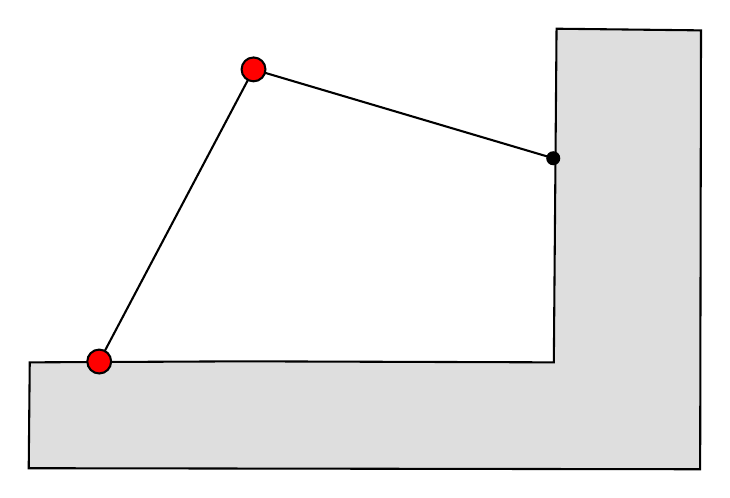
\begin{tikzpicture}[x=0.75pt,y=0.75pt,yscale=-1,xscale=1]
%uncomment if require: \path (0,300); %set diagram left start at 0, and has height of 300

%Straight Lines [id:da511009501867824] 
\draw    (150.25,190.35) -- (224.6,49.6) ;
%Straight Lines [id:da8106680503102979] 
\draw    (224.6,49.6) -- (369,92.4) ;
%Shape: Polygon [id:ds12621320375323086] 
\draw  [fill={rgb, 255:red, 222; green, 222; blue, 222 }  ,fill opacity=1 ] (440.2,30.8) -- (370.6,30) -- (369.29,190.75) -- (219.79,190.25) -- (116.79,190.75) -- (116.29,241.75) -- (439.79,242.25) -- cycle ;
%Shape: Circle [id:dp8262097043760679] 
\draw  [fill={rgb, 255:red, 0; green, 0; blue, 0 }  ,fill opacity=1 ] (366.13,92.4) .. controls (366.13,90.81) and (367.41,89.53) .. (369,89.53) .. controls (370.59,89.53) and (371.88,90.81) .. (371.88,92.4) .. controls (371.88,93.99) and (370.59,95.28) .. (369,95.28) .. controls (367.41,95.28) and (366.13,93.99) .. (366.13,92.4) -- cycle ;
%Shape: Circle [id:dp2680036705913309] 
\draw  [fill={rgb, 255:red, 255; green, 0; blue, 0 }  ,fill opacity=1 ] (144.5,190.35) .. controls (144.5,187.17) and (147.07,184.6) .. (150.25,184.6) .. controls (153.43,184.6) and (156,187.17) .. (156,190.35) .. controls (156,193.53) and (153.43,196.1) .. (150.25,196.1) .. controls (147.07,196.1) and (144.5,193.53) .. (144.5,190.35) -- cycle ;
%Shape: Circle [id:dp33456176340238253] 
\draw  [fill={rgb, 255:red, 255; green, 0; blue, 0 }  ,fill opacity=1 ] (218.85,49.6) .. controls (218.85,46.42) and (221.42,43.85) .. (224.6,43.85) .. controls (227.78,43.85) and (230.35,46.42) .. (230.35,49.6) .. controls (230.35,52.78) and (227.78,55.35) .. (224.6,55.35) .. controls (221.42,55.35) and (218.85,52.78) .. (218.85,49.6) -- cycle ;




\end{tikzpicture}
